\section{\eigendocs{}}\label{sec:evaluation-eigendocs}
% number of components
In order to determine the optimal number of components used for \eigendocs{} the cumulative explained variance and the reconstruction error were plotted 
as displayed in \autoref{fig:det_n_comp} from \autoref{subsec:eigenface}.
The first plot indicated that 90\% of the variance is explained by 95 components.
Usually, that would have been the number of dimensions of the subspace onto which the documents would have been projected.
However, when working with cluster algorithms like \ac{optics} the number of dimensions should be reduced even further to achieve valid clusters.
Therefore the second approach was used.
The second plot showed the reconstruction error with respect to different numbers of components.
\textcolor{red}{"knees"} were visible at 10 and 13.
Since visual inspection accounted for the fact that the decline of the reconstruction error after 13 declined more than after 10, the number of components chosen is 13.

% results
The results of the \eigendocs{} algorithm are displayed in \autoref{fig:preprocessed_docs_eigendocs}.

\begin{figure}[htp] % htp = hier (h), top (t), oder auf einer eigenen Seite (p).
    \centering
    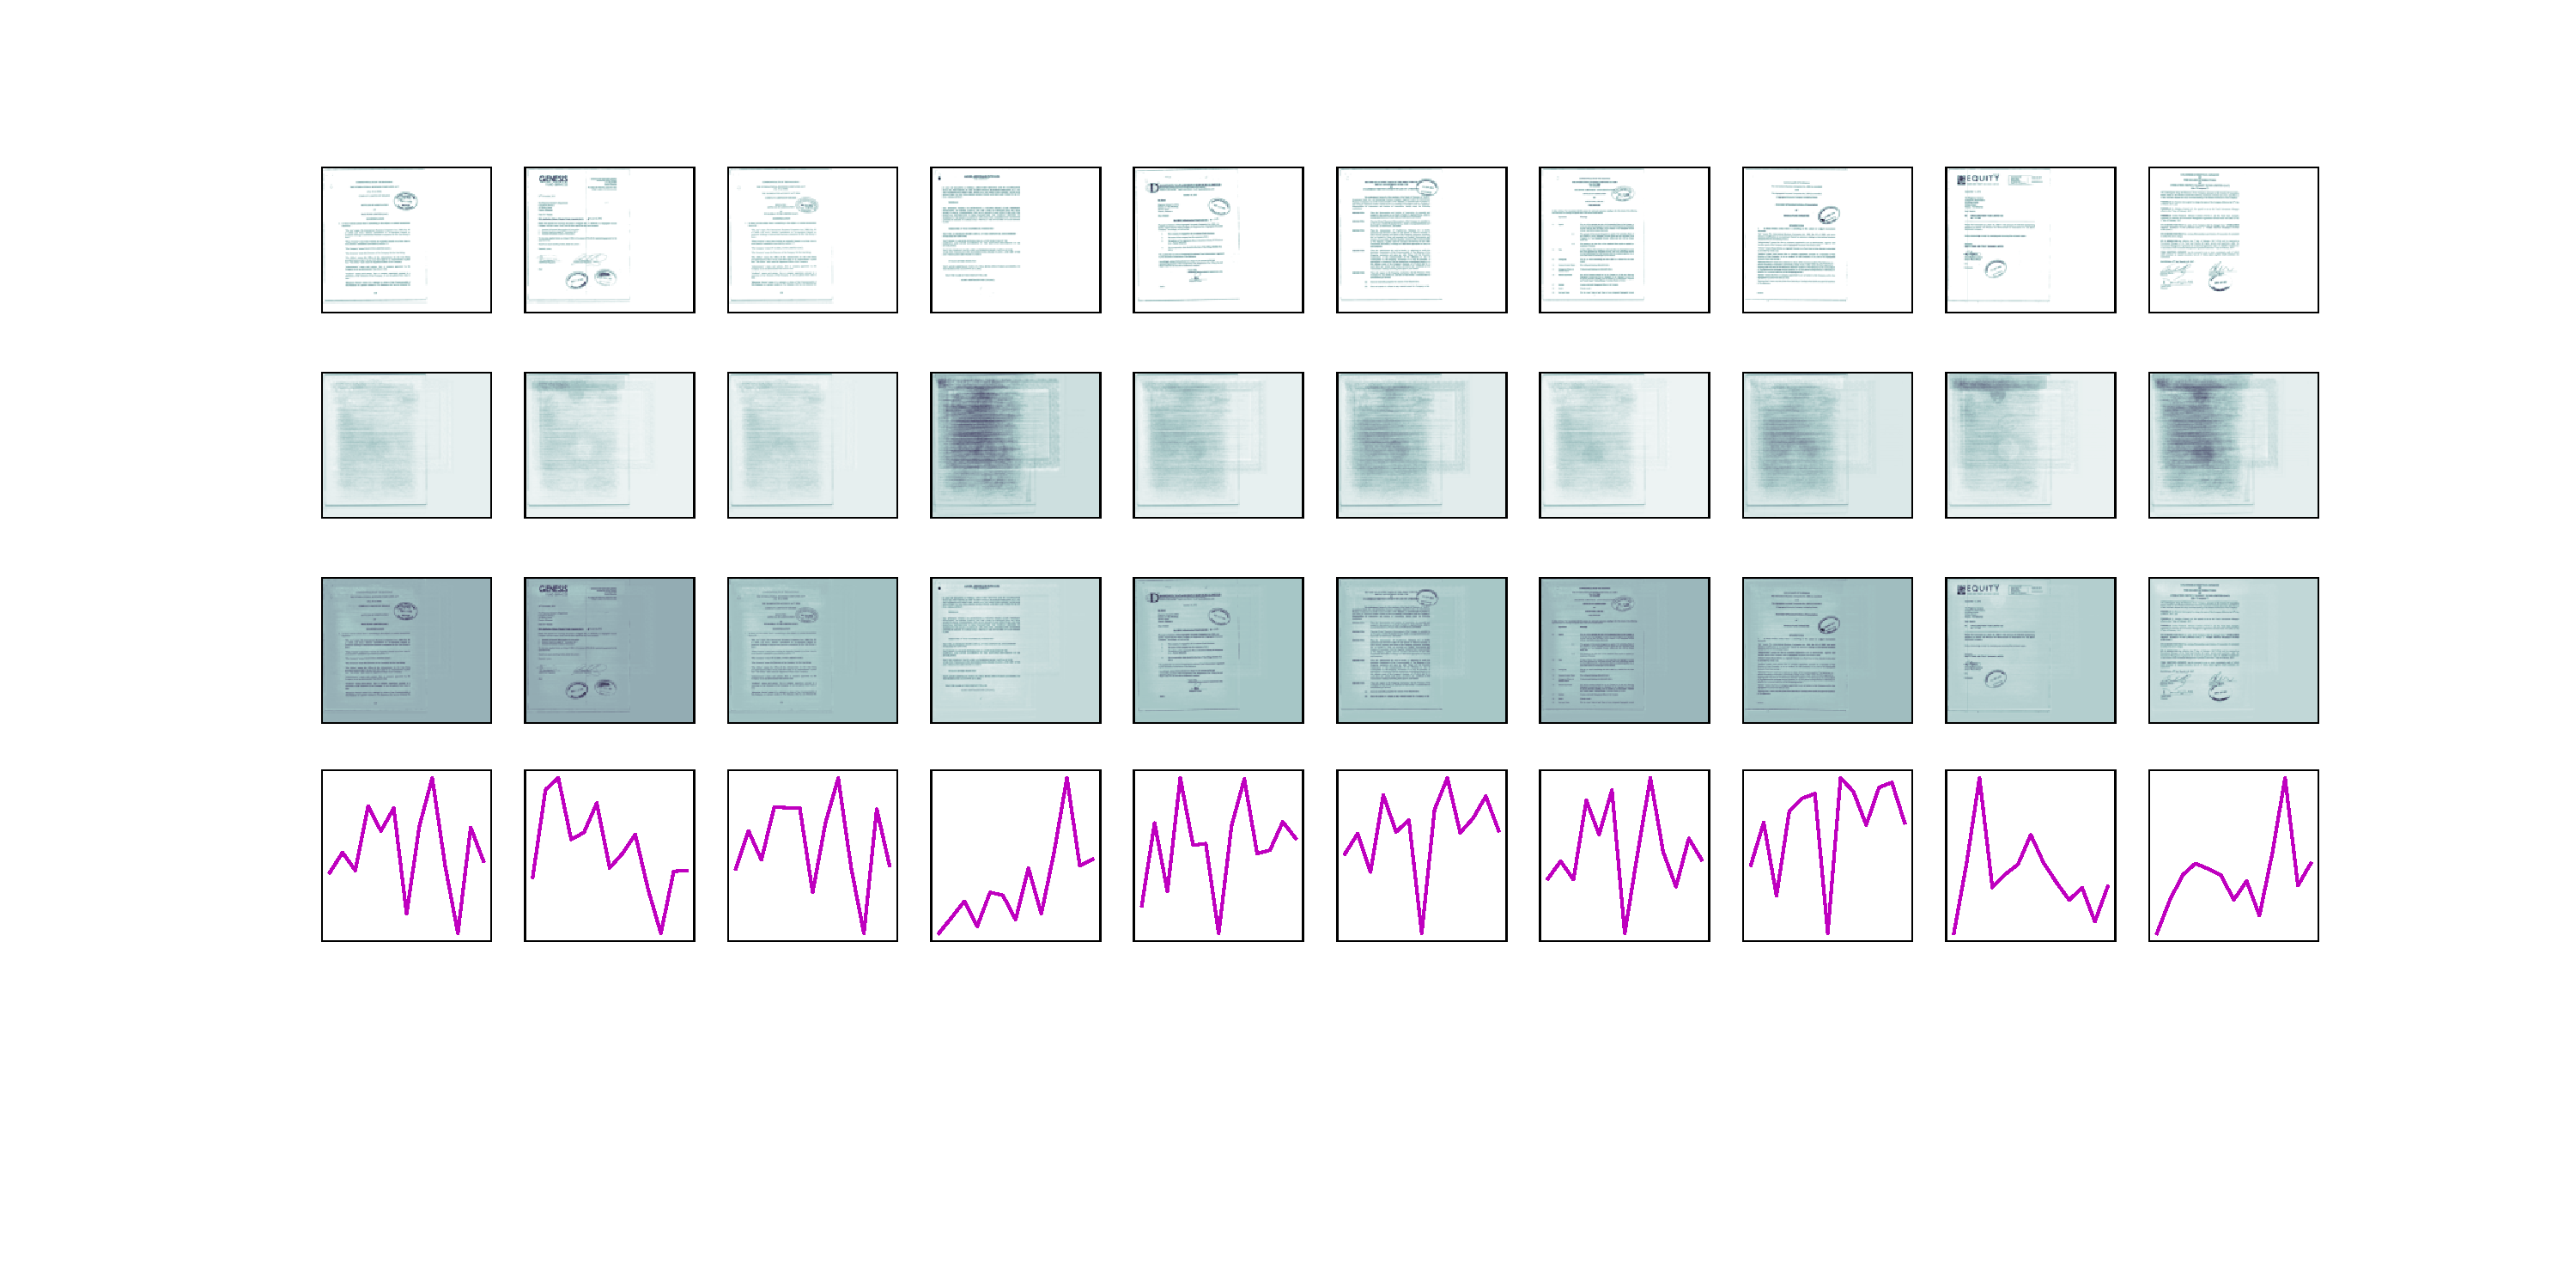
\includegraphics[width=0.7\textwidth]{images/Eigendocs/transformation/eigendocs_13dims.pdf}
    \caption{The first 10 preprocessed documents of the dataset.
    The original images are displayed in the first row.
    The second row shows the reconstructed images using the compressed images from the fourth row.
    The third row shows the reconstruction error, i.e. the difference between the reconstructed and the original image.
    The last row presents the greyscale values of the compressed 13-dimensional image as a line.
    }
    \label{fig:preprocessed_docs_eigendocs}
\end{figure}


\textcolor{red}{documents saved as images in .png format, bad quality to minimize the size of the database
when querying db, top image results looked similar, which is how the idea of this section arose}

The preprocessing of the documents using \eigendocs{} should have encoded information about the dimensionality of the images 
under the assumption the selection of documents is representative.
However, this assumption is not valid since there are bigger document images.
Therefore, the idea of incorporating this information is not entirely implemented.